\subsection{Consistency checking of Type-1 Instances} 
\label{sec:type1consist}

Consistency checking of class expressions such as those of
Definition~\ref{def:ce} is known to be {\em P-space} complete, so that
determening whether a Type-1 instance has a model requires radically
different checking techniques than Type-0 instances.  Specialized
theorem-provers are generally implemented to check consistency of
class expressions.  These provers may use based on structural
subsumption techniques (e.g. as used in CLASSIC~\cite{PMBRB91},
LOOM~\cite{MacB94} and GRAIL~\cite{RBGHNS97}); tableaux
construction~\cite{HoPS99}(redo Bibs); or stable model
generation~\cite{Swif03} --- the CDF theorem prover is based on the
last technique.

At a high level, the CDF prover first translates a class expression
$CE$ to a formula $\psi$ in an ontology language according to
Definition~\ref{def:fot}.  It then attempts to construct a model for
$\psi$: if it succeeds $CE$ is consistent, otherwise $CE$ is
inconsistent (since the prover is assumed to be complete).  The CDF
prover has access to the relational and class hierarchies of a CDF
instance during its execution.  As a result, only the principle
classes and relations of an identifier (Definition~\ref{def:redund})
need be entered in class expressions.  Further details of how the CDF
prover checks consistency of class expressions are beyond the scope of
this paper; here we focus on how the prover is integrated with the CDF
system.  In particular, when a CDF Type-1 instance is checked, the
instance must be translated into either a class expression or a
formula in an ontology language before it can be sent to the CDF
prover.  Due to the high worst-case complexity of consistency
checking, input strings to the prover should be kept as small as
possible.  The CDF system accomplishes this by translating information
about a given CDF identifier into a series of {\em local} class
expressions, sending each local class expresion to the CDF prover,
then producing and checking other local class expressions as needed.
We describe the process through a detailed example before turning to a
more formal description of the concepts and algorithms used.

%------------------------------------------------------------------------------------
\begin{example} \rm \label{ex:type1cc}
Consider the object {\tt oid(inconSuture)}, introduced in
Example~\ref{ex:ce1}.  As {\tt oid(inconSuture)} is an element of {\tt
cid(absorbableSuture)}, the facts
%-------------
{\small
\begin{tabbing}
fooo\=foooo\=foo\=foo\=foooooooooooooooooooooooooooo\=oooooooooo\=\kill
\> (1) \> {\tt allAttr(oid(inconSuture),rid(needleDesign),cid(needleDesignType))} 
\\
\> (2) \> {\tt isa(oid(inconSuture),cid(absorbableSuture)} 
%\> (2.1) \> {\tt isa(oid(inconSuture),cid(sutures)} \\
%\> (2.2) \> {\tt isa(oid(inconSuture),cid(woundCareProducts)}  \\
%\> (2.3) \> {\tt isa(oid(inconSuture),cid(medicalEquipment)} \\
%\> (2.4) \> {\tt isa(oid(inconSuture),cid('CDF Classes')}
\end{tabbing}
}
%-------------
\noindent
hold (cf. Example~\ref{ex:suture2}).  as does
%-------------
{\small
\begin{tabbing}
fooo\=fooo\=foo\=foo\=fooooooooooooooooooooooooooooooo\=oooooooo\=\kill
\> (3) \> {\tt allAttr(oid(inconSuture),rid(hasPointStyle),cid(pointStyle)) } \\
\> (4) \>{\tt hasAttr(oid(inconSuture),rid(hasPointStyle),cid(pointStyle)) }
\end{tabbing}
}
%-------------
\noindent
(cf. Example~\ref{ex:hasAttr}).  Furthermore, from Example~\ref{ex:maxAttr}
%-------------
{\small
\begin{tabbing}
foo\=fooo\=foo\=foo\=foo\=foo\=foooo\=foooooooooooooooo\=\kill
\> (5) \>{\tt allAttr(oid(inconSuture),rid(hasImmedPart),cid(absSutPart)) } \\
\> (6) \>{\tt hasAttr(oid(inconSuture),rid(hasImmedPart),cid(absSutNeedle)) } 
%\> (7) \>{\tt hasAttr(oid(inconSuture),rid(hasImmedPart),cid(absSutThread)) } 
\end{tabbing}
}
%-------------
\noindent
all hold, along with 
%-------------
{\small
\begin{tabbing}
foo\=fooo\=foo\=foo\=foo\=foo\=foooo\=foooooooooooooooo\=\kill
\> (7) \> {\tt hasAttr(oid(inconSuture),rid(hasImmedPart),oid(inconThread)) }
\end{tabbing}
}
%--------------
\noindent
from Example~\ref{ex:ce1}.  Other facts hold, but they are redundant
(Definition~\ref{def:redund}) given (1)-(7) above.  In general, to
produce a local class expression for an object or class $Id_1$, in a CDF
instance $\cO$, we begin by collecting an irredundant set $\cS$ of CDF
facts whose first argument is $Id_1$.

Next, since the class expressions of Definition~\ref{def:ce} do not
reference objects, each object identifer $Id_1$ is translated to a
singleton class whose interpretation will be $\{Id_1\}$.  Thus for
this example, we create a new class, {\tt cid(inconSuture)} containing
only {\tt oid(inconSuture)}.  Recall that the inheritance mechanisms
of CDF treat the construct $unique(cid(I))$ as $oid(I)$, so that the
information about the inheritance hierarchy will be preserved.  A
similar transformation is made to {\tt oid(inconThread)} to produce
the {\em local class formula} $\phi_{cid(inconSuture)}[X_0]$:
%-------------
{\small
\begin{tabbing}
foo\=fooo\=foo\=foo\=foo\=foo\=foooo\=foooooooooooooooo\=\kill
\> $elt(X_0,cid(inconSuture)) \wedge 
	\forall X_1 [elt(X_1,cid(inconSuture)) \Ra X_1 = X_0]$ \\
\> $\forall X_1 [rel(X_0,rid(needleDesign),X_1)
	\Ra elt(X_1,cid(needleDesignType))] \wedge$ \\
\> $\forall X_1 [rel(X_0,rid(hasPointStyle),X_1) 
	\Ra elt(X_1,cid(pointStyle))] \wedge$ \\
\> $\exists X_1 [rel(X_0,rid(hasPointStyle),X_1) 
	\wedge elt(X_1,cid(pointStyle))] \wedge$ \\
\> $\forall X_1 [rel(X_0,rid(hasImmedPart),X_1) 
	\Ra elt(X_1,cid(absSutPart))] \wedge$ \\
\> $\exists X_1 [rel(X_0,rid(hasImmedPart),X_1) 
	\wedge elt(X_1,cid(absSutNeedle))] \wedge$ \\
\> $\exists X_1 [rel(X_0,rid(hasImmedPart),X_1) 
	\wedge elt(X_1,cid(inconThread)) \wedge 
		\forall X_2 [elt(X_2,cid(inconThread)) \Ra X_1 = X_2]$  
\end{tabbing}
}
%--------------
\noindent
Note that $\phi_{cid(inconSuture)}[X_0]$ is logically equivalent to
$C_{inconSuture}[X_0]^{\cI}$ (Definition~\ref{def:fot}) where
$C_{inconSuture}$ is the (local) class expression
%-------------
{\it {\small
\begin{tabbing}
foo\=fooo\=foo\=foo\=foo\=foo\=foooo\=foooooooooooooooo\=\kill
\> unique(cid(inconSuture)),  \\
\> all(rid(needleDesign),cid(needleDesignType)), \\
\> all(rid(hasPointStyle),cid(pointStyle)), \\
\> exists(rid(hasPointStyle),cid(pointStyle)), \\
\> all(rid(hasImmedPart),cid(absSuturePart)), \\
\> exists(rid(hasImmedPart),cid(absSutureNeedle)), \\
\> exists(rid(hasImmedPart),unique(cid(inconThread)))
\end{tabbing}
} }
%--------------
\noindent
A {\em local class structure} for $C_{inconSuture}$ is depicted by the
following predicates.
%--------------
{\it {\small
\begin{tabbing}
foo\=foooooooooooooooooooooooooo\=fooooo\=fooooooooooooooooooooooooooooooo\=\kill
\> elt(d$_0$,cid(inconSuture)) 
		\> \> elt(d$_1$,cid(pointStyle)) \\
\> rel(d$_0$,rid(hasPointStyle),d$_1$) \\
\> elt(d$_2$,cid(absSutureNeedle))
	\> \> elt(d$_3$,cid(inconThread)) \> elt(d$_3$,cid(absSuturePart)) \\
\> rel(d$_0$,rid(hasImmedPart),d$_2$) 
		\> \> rel(d$_0$,rid(hasImmedPart),d$_3$) 
\end{tabbing}
} }
%--------------
\noindent
For simplicity, the presentations of structures in this paper describe
only the principle classes to which an individual $d$ belongs and the
principle relations between individuals (Definition~\ref{def:redund}).
For visualization purposes, the above structure is also portrayed via
a structure graph in Figure~\ref{fig:struct1}~\footnote{Structure
graphs are used in this paper only for expository purposes,
\cite{Swif03} provides definitions of a structure graph for ontology
languages.}.  The vertices of a structure graph correspond to the
individuals in the structure labelled with the principle classes to
which the individuals belong, along with any uniqueness constraints
The edges of a structure graph represent binary relations in the
structure and are labelled with the name of the relation
%--------------
\begin{figure}[htbp] 
\centering {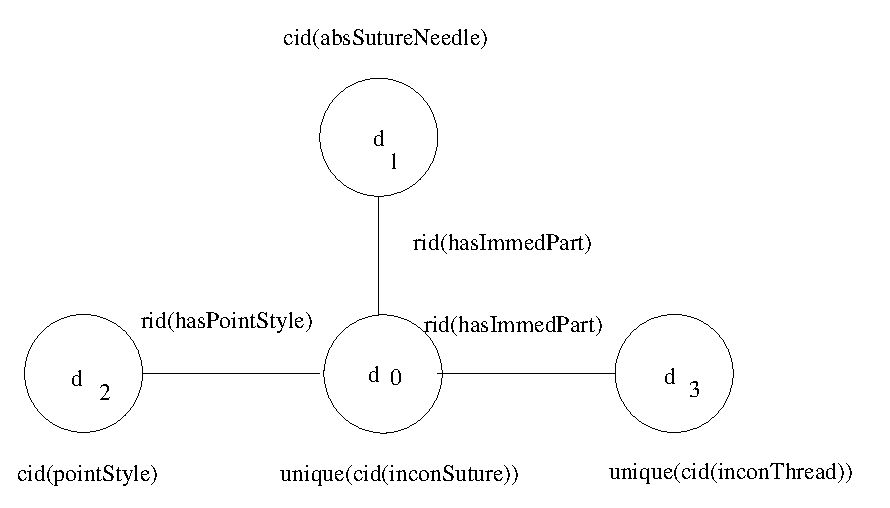
\epsfig{file=Figures/struct1.eps,width=0.55\textwidth}}
\caption{A Structure Graph for $C_{inconSuture}$}
\label{fig:struct1}
\end{figure}
%--------------

Of course, local class expressions, formulas and structures omit much
information about an ontology theory.  Thus, while the local class
expression $C_{inconSuture}$ is consistent, the CDF instance as a
whole is not, as indicated in Example~\ref{ex:ce1}.  There are two
ways in which inconsistency can arise: in the first case, a local
class formula may be inconsistent in itself; in the second, an
individual in a local class structure may be an element of several
classes whose class formulas, cojoined together, are inconsistent with
one another.  We therefore must continue to check consistency of each
set of classes to which each element in the structure belongs.  As a
next step, we consider the consistency of {\tt
unique(cid(inconThread))}; by a process similar to that above, its
local class expression is derived as:
%-------------
{\it {\small
\begin{tabbing}
foo\=fooo\=foo\=foo\=foo\=foo\=foooo\=foooooooooooooooo\=\kill
\> unique(cid(inconThread)),\\
\>
exists(rid(hasMaterial),cid(gut)),exists(rid(hasMaterial),cid(polyglyconate)),\\
\> atMost(1,rid(hasMaterial),cid(material))
\end{tabbing}
} }
%--------------
A local class structure for $C_{inconThread}$ is shown within the
dotted line of Figure~\ref{fig:struct2}.  As we will make more precise
below, two local class structures are amalgamated by identifying
individuals with the same principle classes and uniqueness
constraints, so that the whole structure of Figure~\ref{fig:struct2}
indicates the amalgamation of local class structures for both {\tt
unique(cid(inconSuture))} and {\tt unique(cid(inconThread))}.

%--------------
\begin{figure}[htbp] \label{fig:struct2}
\centering {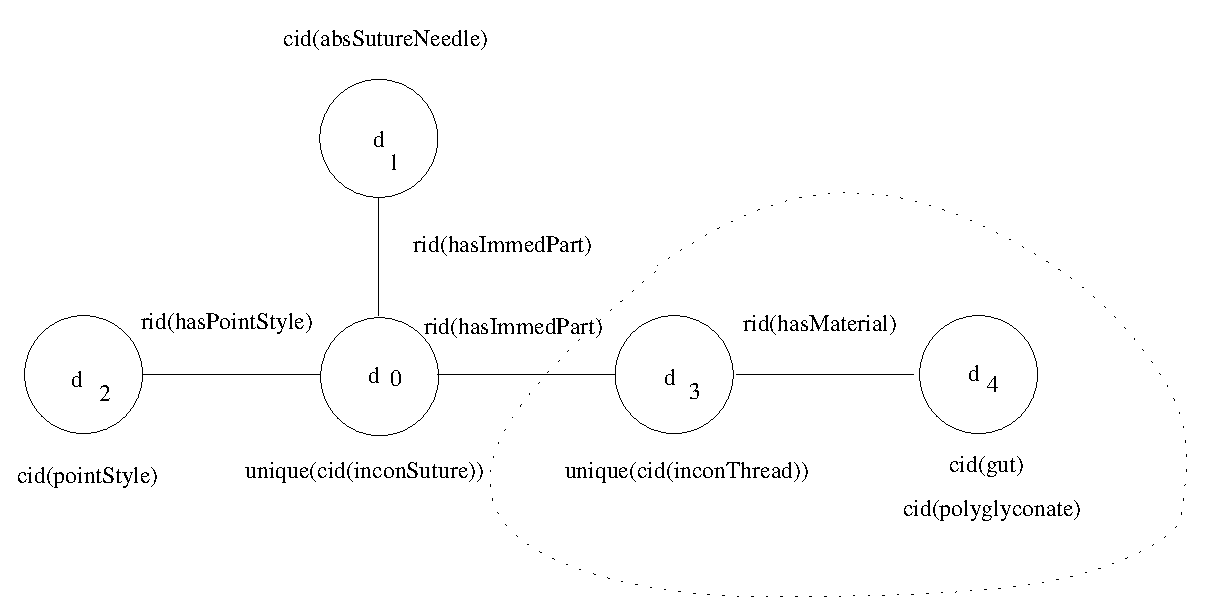
\epsfig{file=Figures/struct2.eps,width=0.75\textwidth}}
\caption{A Structure Graph for $C_{inconSuture,inconThread}$}
\end{figure}
%--------------
Due to the $atMost$ number restriction in $C_{inconThread}$ the
individual $d_4$ in its local class structure belongs to two principle
classes: {\tt cid(gut)} and {\tt cid(polyglyconate)}.  Accordingly we
must now construct the local class expression
$C_{gut,polyglyconate}$, i.e.
%-------------
{\it {\small
\begin{tabbing}
foo\=fooo\=foo\=foo\=foo\=foo\=foooo\=foooooooooooooooo\=\kill
\> cid(gut),cid(polyglyconate),not cid(gut) 
\end{tabbing}
} }
%--------------
\noindent
which is clearly inconsistent.
\end{example}

%------------------------------------------------------------------------------------
\begin{figure}[htbp]
\longline
{\sf
\begin{tabbing}
foo\=foo\=foo\=foo\=foo\=foo\=foooo\=foooooooooooooooo \=fooooooooo\=\kill

\> \underline{getRelevantFacts($Id_{in}$)} \\
\> \> If $Id_{in} = unique(cid(Id_1))$ then $Id = oid(Id_1)$ else $Id = Id_{in}$ \\
\> \> Let $\cO_{Id}$ be the set of $f \in \cO$ such that  \\
\> \> \> $f$ is of the form $allAttr(Id1,R,C2)$, 
$hasAttr(Id1,R,C2)$, $maxAttr(Id1,R,C2,N)$,  \\
\> \> \> \> \> $minAttr(Id1,R,C2,N)$ or $necessCond(Id1,E)$, and  $\cO
			\models_{inh} isa(Id,Id1)$ \\ 
\> \> \> or $f$ is of the form $H \Leftarrow CE$, and  no class
	identifier occurs directly in $f$ \\
\> \> \> or $f$ is of the form $H \Leftarrow CE$ and for some class identifer
	$Id1$ that occurs directly in $f$,  \\
\> \> \> \> \>  $\cO \models_{inh} isa(Id,Id1)$ \\
\> \> Return an irredundant basis for $\cO_{id}$ 
\> \> \> \> \> \> \>		{\rm /* cf. Definition~\ref{def:redund} */}\\
%------------------------------------------------------------------------------------
\ \\
\>  \underline{LocalClassExpression($Id$)}  \\
\> \> Let $\cF = getRelevantFacts(Id)$ \\
\> \> $CE = Id$ \\
\> \> For each $f \in \cF$ \\
\> \> \> If $f = allAttr(Id,R,C2)$, then $CE_f = all(R,C2)$ else \\
\> \> \> If $f = hasAttr(Id,R,C2)$, then $CE_f = exists(R,C2)$ else \\
\> \> \> If $f = maxAttr(Id,R,C2,N)$, then $CE_f = atmost(R,C2)$ else \\
\> \> \> If $f = minAttr(Id,R,C2,N)$, then $CE_f = atleast(R,C2)$ else
									\\
\> \> \> If $f = necessCond(Id,vid(Expr))$, then $CE_f = Expr$ \\
\> \> \> If $f = H \Leftarrow CE$, then $CE_f = (H \vee \neg CE)$ \\
\> \> \> $CE = CE,CE_f$ \\
\> \> For each object identifier $O = oid(Oid)$ in $CE$ \\
\> \> \> Replace all occurrences of $O$ in $CE$ by $cid(Oid)$ \\
\> \> \> Let $\cP$ be a conjunction of all the principle classes to
	which $O$ belongs \\
\> \> \> $CE = CE,\cP,unique(Oid)$  \\
\> \> return CE \\
\\
%------------------------------------------------------------------------------------
\>  \underline{LocalClassFormula($Id$)}  \\
\> \> Let $\cF = getRelevantFacts(Id)$ \\
\> \> If $Id$ is a class identifier, CF = $elt(X_0,Id)$ \\
\> \> Else If $Id$ is an object identifier $oid(I)$ \\
\> \> \> CF = $elt(X_0,cid(I)) 
	\wedge \forall X_1 [elt(X_1,cid(I)) \Ra X_1 = X_0]$ \\
\> \> while $\cF$ is non-empty \\
\> \> \> remove a new fact $f$ from $\cS$ \\
\> \> \> If $f = allAttr(Id,R,Id_2)$, then 
	$CF_f = \forall X_1 [rel(X_0,R,X_1) \Ra elt(X_1,Id_2)]$ \\
\> \> \> If $f = hasAttr(Id,R,Id_2)$, then 
	$CF_f = \exists l X_1 [rel(X_0,R,X_1) \wedge elt(X_1,Id_2)]$ \\
\> \> \> If $f = maxAttr(Id,R,Id_2)$, then 
	$CF_f = \exists^{\leq N} [rel(X_0,R,X_1) \Ra elt(X_1,Id_2)]$ \\
\> \> \> If $f = minAttr(Id,R,Id_2)$, then 
	$CF_f = \exists^{\geq N} [rel(X_0,R,X_1) \Ra elt(X_1,Id_2)]$ \\
\> \> \> If $f = necessCond(Id,vid(Expr))$, then $CE_f = Expr^{\cI}[X_1]$ \\
\> \> \> If $f = H \Leftarrow CE$, then $CE_f = (H \vee \neg CE)^{\cI}[X_0]$ \\
\> \> \> If $Id_2$ is an object identifier $O = oid(I)$ \\
\> \> \> \> Replace $Id_2$ in $CF$ by $cid(I)$ \\
\> \> \> \> Let $\cP$ be the set of principle classes for $Id_2$ in $\cO$ \\
\> \> \> \> $CO = \bigwedge_{Cid \in \cP} elt(X_1,Cid) $ \\
\> \> \> \> $CF = CF \wedge CO \wedge 
		\forall X_2 [elt(X_2,cid(I)) \Ra X_1 = X_2] $\\
\> \> return $CF$
\end{tabbing}
}
\caption{Local Class Expressions and Identifiers}
\label{fig:lcelcf}
\longline
\end{figure}
%------------------------------------------------------------------------------------

\paragraph*{Local Class Expressions and Formulas}
We now turn to the formalization of the algorithm sketched in
Example~\ref{ex:type1cc}.  To start, we begin by formalizing the
construction of local class expressions and formulas in
Figure~\ref{fig:lcelcf}.  Construction of both local class expressions
for an identifier $Id$ begins with obtaining all of the facts relevant
to $Id$, as described by the routine {\sf getRelevantFacts($Id$)}.
This routine begins with a transformation that is purely technical.
In most parts of CDF an object is designated via an object identifier
$oid(I)$, but in class expressions an object is cast into a singleton
set, $unique(cid(I))$.  The first line simply ensures that both
designations are handled in the same manner.  {\sf getRelevantFacts}
then uses first argument inheritance to obtain all {\tt allAttr/3},
{\tt hasAttr/3}, {\tt minAttr/4}, {\tt maxAttr/4} and {\tt
necessCond/2} facts.  {\tt isa/2} facts are not needed because the CDF
prover and translation algorithm use the inheritance hierarchy of a
CDF instance as a ``background theory'' as mentioned above.  The
absence of {\tt isa/2} facts in local class expressions and formulas
is accounted for in the lemmas and theorem below. It next finds
relevant sufficiency rules using those class identifiers that occur
directly in those rules (Definition~\ref{def:suffic}).  And finally,
it finds an irredundant basis for that set.

A local class expression for a given class or object identifier, $Id$,
is constructed by the routine {\sf LocalClassExpression(Id)}, which
begins by calling {\sf getRelevantFacts($Id$)} to obtain the set of
facts $\cF$ relevant to $Id$.  Each fact in $\cF$ is translated to a
class expression, and the class expressions cojoined together to form
a class expression $CE$.  If an object identifier, say $oid(I)$ occurs
in $CE$, all occurrences of $oid(I)$ are replaced by $cid(I)$.  In
addition, $cid(I)$ is made into a singleton class by cojoining the
constructor $unique(I)$ to $CE$ (Definition~\ref{def:ce}).  Note that
$cid(I)$ is guarenteed not to occur in $\cO$ by Axiom 1.  Since
$cid(I)$ is newly created, $\cO$ will not contain {\tt isa/2}
relations for it; thus the principle classes to which $cid(I)$ belongs
must also be cojoined with $CE$.  Note that predicates of the form
{\tt classHasAttr/3} are not used to construct the local class
expression: this is because {\tt classHasAttr/3} defines
class-relations for a class, which will not cause inconsistency with
the relations of an Ontology Theory.  Also note that since $\cO$ is
assumed to be acceptable, product classes and objects do not need to
be handled separately in forming a class expression.  Their
specialized inheritance is handled by the CDF inheritance mechanisms,
and does not require special mechanisms by the CDF prover, or the
routines of Figure~\ref{fig:type1cc}.

%--------------------------------------
\mycomment{
It is easy to see from the translation axioms that if, say the fact
$f$ is {\tt hasAttr(Cid,r,Cid1)}, the $\phi_f[X_0]$ is logically
equivalent to $exists(r,Cid1)[X_0]^{\cI}$ of Definition~\ref{def:fot}.
Translations for other cases are given in Figure~\ref{fig:type1cc}.
If $Id_1$ is a class, then $Id_1$ itself is added to the local class
expression.  All of the superclasses of $Id_1$ will be available to
the prover as it attempts to construct a model for the class
expression.  
}
%--------------------------------------

Local class formulas are produced in an analogous way by {\sf
localClassFormula(Id)}.  Assume for a moment that a CDF instance
$\cO_{class}$ contains no object identifiers, and let $Cid$ be a class
identifier.  SInce $\cO_{class}$ is assumed to be well-typed, applying
the translation axioms to each fact $f$ in $\cO_{Cid}$ gives a
conjunction of formulas that is $Th(\cO)$-equivalent to:
\[ 
\bigwedge_{f \in \cO_{cid}} \forall X_0 [elt(X_0,Id) \Ra \phi_f[X_0]]
\]
adding Axiom~\ref{ax:nonnull}, we get 
\[ 
\phi_{Cid} = \exists X_0 [elt(X_0,Cid)] \wedge \forall X_0 [elt(X_0,a) \Ra
				\bigwedge_{f \in \cO_{cid}} \phi_f[X_0]] 
\]
which is logically equivalent to 
\[ 
\exists X_0 [elt(X_0,Cid)] \wedge \bigwedge_{f \in \cO_{cid}} \phi_f[X_0]] 
\]
or 
\[ 
\exists X_0 [localClassFormula(Cid)] 
\]

In a more general case, $\cO$ will also contain object identifiers,
and the above argument, while it becomes more complicated, remains
essentially the same, so that the local class formula is
$TH(\cO)$-equivalent to the instance axioms applied to all facts in
{\sf getRelevantFacts($Id$)}.  In addition, it is an easy induction to
show that for any identifier $Id$ in a CDF instance, {\sc
localClassFormula(Id)} is logically equivelent to
$localClassExpression(Id)^{\cI}[X_0]$
%
%--------------------------------------------------------------------------
\mycomment{
Similarly if $f$ is {\tt allAttr/3} $\phi_f[X_0]$ is equivalent to the
translation of an $all$ constructor via Definition~\ref{def:fot}, and
so on for each CDF predicate type: {\tt isa/2} to the atomic class
name constructor, {\tt minAttr/3} to $atLeast$, and {\tt maxAttr/3} to
$atMost$, and {\tt necessCond/2} maps directly to a class expression.
Thus, for a given fact $f$, {\sf ce\_ify(f)} is taken to denote the
class expression such that
\[
\exists X_0 [elt(X_0,Cid) \wedge \phi_f[X_0] ]
\equiv 
\exists X_0 [elt(X_0,Cid) \wedge ce\_ify(f)[X_0]^{\cI} ]
\] }
%--------------------------------------------------------------------------
%
Details can be added to this argument to show: 

%--------------------------------------------------------------------------
\begin{lemma} \label{lem:localce}
Let $\cO$ be a well-typed, acceptable CDF instance, $Id$ be an object
or class identifier in $\cO$, $\cO_{Id}$ be {\sf
getRelevantFacts($Id$)}, and $\cO_{isa}$ be the {\tt isa/2} facts
in $\cO$.
\begin{itemize}
\item $TH(\cO_{Id} \cup \cO_{isa}) \vdash \cO_{Id}^{\cI}
\leftrightarrow \exists X_0 [localClassFormula(Id)] $
\item 
%$(\cO_{Id} \wedge \cO_{isa})^{\cI}$ has a model iff $(Class_{Id}
%\wedge \cO_{isa})^{\cI}$ has a model.
$TH(\cO_{Id} \cup \cO_{isa}) \vdash \cO_{Id}^{\cI}
\leftrightarrow \exists X_0[localClassExpression(Id)]^{\cI}$
\end{itemize}
\end{lemma}
%--------------------------------------------------------------------------

\paragraph*{Combining Local Class Formulas to Check Consistency}
The algorithm for checking consistency of an object or class
identifier $Id$ in a CDF instance $\cO$ is presented schematically in
Figure~\ref{fig:type1cc}.  We assume that $\cO$ is well-typed and
acceptable.  The algorithm begins with a call {\sf
checkIdConsistency(\{$Id$\})}.  As indicated in the previous
discussion, {\sf checkIdConsistency(\{$Id$\}} first transforms
information about $Id$ into a local class expression; then checks
consistency of the local class expression, and constructs new local
class expressions as needed.  Note that {\sf
localClassExpression($Id$)} automatically transforms object
identifiers into classes with uniqueness constraints, so {\sf
checkIdConsistency(\{$Id$\})} can be applied to object identifiers as
well as class identifiers.  In addition, as Figure~\ref{fig:lcelcf}
indicates, {\sf localClassExpression($Id$)} also handles class
identifiers with uniqueness constraints.

%------------------------------------------------------------------------------------
\begin{figure}[htbp]
\longline
{\sf
\begin{tabbing}
foo\=foo\=foo\=foo\=foo\=foo\=foooo\=foooooooooooooooo \=fooooooooo\=\kill

\> \underline{checkIdConsistency($CSet$)}  \\
\> \> 	{\rm /* Memoized: repeated calls do
		not require repeated execution.  */ }\\
\> \> 	{\rm /* Assume consistency is being checked with respect to a
		well-typed, acceptable CDF instance $\cO$ */} \\
\> \> 	Let $CSExpr$ be $\bigwedge_{Id \in CSet} \{$ 
			LocalClassExpr($Id$) $\}$,  \\
\> \> 	If checkCeConsistency($CSExpr$,$Structure$) succeeds  \\
\> \> \> 	    checkContexts($Structure$) \\
\> \>     Else emit cdf warning and abort \\
\\
\> \underline{checkCeConsistency($ClassExpr$,$Structure$)} \\
\> \> {\rm /*  Call to CDF prover: checks consistency of a class
	         expression, returing a $\cL_O$ structure */} \\
\\
\> \underline{checkContexts($Structure$)}  \\
\> \> For each individual $elt$ in $Structure$ \\
\> \> \> If $elt$ belongs to a class with a non-empty set $\cC$ of
			uniqueness constraints \\
\> \> \> \> Set $\cP$ to $\cC$ along with any other principle classes to
		which  $elt$ belongs in $Structure$ \\ 
\> \> \> Otherwise, Set $\cP$ be the set of 
		principle classes to which $elt$ belongs in $Structure$ \\ 
\> \> \> checkIdConsistency($\cP$) \\
\end{tabbing}
}
\caption{Schematic Algorithm for Checking Consistency of Type-1 instances}
\label{fig:type1cc}
\longline
\end{figure}
%------------------------------------------------------------------------------------

Once {\sf LocalClassExpr/1} has been used to transform a (set of)
identifiers into a local class expression, the class expression is
checked for consistency via the CDF prover ({\sf
checkCeConsistency/2}).  If the class expression is consistent, {\sf
checkCeConsistency/2} will produce a structure $Structure$, and the
predicate {\sf checkContexts/1} will check each individual $elt$ in
$Structure$ to determine the {\em context} of $elt$ in $Structure$.
The context of $elt$ contains the principle classes to which $elt$
Uniqueness constraints must be passed along to the next invocation of
{\sf checkConsistency/1} to ensure that models are properly
constructed.

The top-level predicate, {\sf checkIdConsistency/1} is called for
each such context.  Since {\sf checkIdConsistency/1} is memoized,
it will actually check consistency at most once for each context.
Since each context depends only on a set of principle classes, and CDF
instances are defined to be finite (Definitions~\ref{def:ids}
and~\ref{def:type1}), there are a finite set of contexts possible for
a finite CDF instance, and the algorithm will terminate~\footnote{We
note that the omission of inverse relations is crucial to the design
of the algorithms in FIgure~\ref{fig:type1cc}.  The use of inverse
relations would create contexts that depend on an elements relation to
other elements in addition to its principle classes.  Under such a
revised definition, an infinite number of might be produced.}.  Note
that this argument is independent of whether identifier ``definition''
is cyclic, i.e. regardless of whether two identifers occur in the
local class expressions of each other.  Thus, while correctness
remains to be shown, we have shown

\begin{lemma}
Let $\cO$ be a Type-1 CDF Instance.  Then for any set S of class or
object identifiers in $\cO$, {\sf checkIdConsistency(S)} will
terminate.
\end{lemma}

Before showing soundness and completeness of {\sf
checkIdConsistency/1}, we illustrate it by its actions in
Example~\ref{ex:type1cc}.  First, a local class expression is
constructed for {\tt oid(inconSuture)}, and in so doing, this
identifier and other object identifiers are made into singleton
classes.  This local class expression is found consistent (its
structure is shown in Figure~\ref{fig:struct1}), and {\sf
checkContexts/1} is called to backtrack through all of its contexts.
In Example~\ref{ex:type1cc}, {\tt unique(cid(inconThread))} is checked
first.  However, construction of $\cM_{unique(cid(inconThread))}$
requires construction of an element $d_4$ whose principle classes
include both $elt(d,cid(gut))$ and $elt(d,cid(polyglyconate))$.  Note
that {\tt cid(gut)} and {\tt cid(polyglyconate)} are both consistent
in themselves, but the class expression ${\tt cid(gut)},{\tt
cid(polyglyconate)}$ is not, so that the structure
$\cM_{unique(cid(inconThread))}$ is not a model of
$\phi_{cid(polyglyconate)} \wedge \phi_{cid(gut)}$.

The following definition introduces is required to formulate
correctness of {\sf checkIdConsistency/1}, and makes use of the
$\vdash_{inh}$ relation (Definition~\ref{def:redund}).  This
terminology is not used outside of this section.
%------------------
\begin{definition}
 Let $\cO$ be a CDF instance.  An identifier $Id$ {\em directly
 depends on} an identifier $Id_{targ}$ if $\cO \vdash_{inh} f$, and
 $f$ is {\tt hasAttr(Id,R,Id$_{targ}$)}, {\tt
 allAttr(Id,R,Id$_{targ}$)}, {\tt maxAttr(Id,R,Id$_{targ}$)}, or {\tt
 minAttr(Id,R,Id$_{targ}$)}; or $f$ is {\tt necessCond(Id,Expr)} and
 {\tt Id$_{targ}$} occurs in $Expr$.  The transitive closure of the
 ``directly depends on'' relation is the ``depends on'' relation.

Let $\cS$ be a set of identifiers.  The {\em subinstance of $\cO$
generated by $\cS$}, $subinst(\cO,\cS)$ is the conjunction of the
translations of {\tt isa/2} facts in $\cO$ along with the local class
formulas for each identifier $S'$ upon which $S \in \cS$ depends.  The
local subinstance of $\cO$ generated by $\cS$ $locinst(\cO,\cS)$ is
the conjunction of translations of {\tt isa/2} facts in $\cO$ along
with the local class formulas for each identifier in $\cS$.
\end{definition}
%------------------

\begin{theorem} \label{thm:type1consist}
Let $\cO$ be a well-typed and acceptable CDF instance, and $Clist$ be
a set of identifiers in $\cO$.  Then {\sf checkIdConsistency(Clist)}
succeeds if and only if $subinst(\cO,\cS)$ has a model.
\end{theorem}

\begin{proof} (Sketch)
As stated before, there are a number of sound and complete algorithms
to check the consistency of class expressions of the sort defined in
Definition~\ref{def:ce}, so that we may assume soundness and
completeness of {\sf checkCeConsistency/2}, and that if it succeeds,
it produces a representation of $Structure$ as a finite data
structure. Furthermore, Lemma~\ref{lem:localce} states the equivalence
between local class expressions and local class formulas, so that {\sf
LocalClassExpr/1} is assured to be correct.  In addition,
Lemma~\ref{lem:localce} allows us to ignore class expressions and
consider only local class formulas in this proof.  Finally, the
correctness of {\sf checkContexts/1} is straightforward, as it
searches through a finite data structure for the different contexts
contained in the structure.

Thus, the proof of correctness focuses on two aspects.  Let $\cS$ be a
set of identifiers, and $\cS = \cS_1 \cup \cS_2$.
\begin{enumerate}
\item $subinst(\cO,\cS)$ has a model $\cM$ iff for each context $Ctxt$
in $\cM$, $locinst(\cO,Ctxt)$ has a model.

The non-trivial portion of this statement is the backward implication
($\Leftarrow$). The main mechanism in proving this consists of showing
that models of two local class formulas can be amalgamated into a
model of their conjunction.  Let $Id_1$ and $Id_2$ be two consistent
class or object identifiers; $\phi_{Id_1}$, and $\phi_{Id_2}$ their
local class formulas; and $\cM_{Id_1}$ and $\cM_{Id_2}$ local class
models.  Figure~\ref{fig:amalg} shows how $\cM_{Id_1}$ and
$\cM_{Id_2}$ can be {\em amalgamated} into a new {\em amalgamated}
structure.  It is straightforward to see that $\cM_{amalg} \models
\exists \phi_{Id1}[X_0]$, and $\cM_{amalg} \models \exists
\phi_{Id_2}[X_0]$, so that $\cM_{amalg} \models \exists
\phi_{Id_1} \wedge \phi_{Id_2}[X_0]$.  This argument can be extended
into a straightforward induction on the number of identifiers in
$\cS$.

\item $\{ I' | \mbox{ there exists } S \in \cS, \mbox{ and } S
\mbox{ depends on } I\}$ is equal to $\{ I' | \mbox{ there exists } S
\in \cS_1, \mbox{ and } S \mbox{ depends on } I\} \cup \{ I' | \mbox{
there exists } S \in \cS_2, \mbox{ and } S \mbox{ depends on } I\}$.

\end{enumerate}
\end{proof}

%--------------
\noindent
Next, we replace occurrences of {\tt oid(inconSuture)} in the above
sentence by the variable $X_0$, and add the conjunct
$elt(X_0,cid(inconSuture))$ 
{\small
\begin{tabbing}
foo\=fooo\=foo\=foo\=foo\=foo\=foooo\=foooooooooooooooo\=\kill
\> $elt(X_0,cid(inconSuture)) \wedge$ \\
\> $\forall X_1 [rel(X_0,rid(hasPointStyle),X_1) 
	\Ra elt(X_1,cid(pointStyle))] \wedge$ \\
\> $\exists X_1 [rel(X_0,rid(hasPointStyle),X_1) 
	\wedge elt(X_1,cid(pointStyle))] \wedge$ \\
\> $\forall X_1 [rel(X_0,rid(hasImmedPart),X_1) 
	\Ra elt(X_1,cid(absSutPart))] \wedge$ \\
\> $\exists X_1 [rel(X_0,rid(hasImmedPart),X_1) 
	\wedge elt(X_1,cid(absSutNeedle))] \wedge$ \\
\> $rel(oid(inconSuture),rid(hasImmedPart),oid(inconThread))$ 
\end{tabbing}
}

\subsection{Type-0 CDF Instances and and Description Logics}
\label{sec:comp} 

Clearly Type-1 CDF instances are at least as expressive as ${\cal
ALCQ}$ description logics, since any ${\cal ALCQ}$ class expression
can be used directly in a {\tt necessCond/2} fact.  To formalize the
relation between Type-0 class expressions and description logics, we
use the definition of an {\em atomic relational CDF instance}.
\begin{definition}
Let $\cO$ be a CDF intance.  $\cO$ is {\em atomic} if it contains no
product identifiers.  $\cO$ is a {\em relational instance} if it
contains no object identifiers, and no {\tt classHasAttr/3}
predicates.
\end{definition}

We also need to formalize the language of class expressions that we
will use.

\begin{definition}
The syntax of an \omsdl{} class expression has the following form, in
which $A$ is an atomic class identifier, $R$ a relation identifer, $N$
a non-negative integer, and $C_1$ and $C_2$ \omsdl{} class expressions.
\[ C \leftarrow A | C_1 \sqcap C_2 | all(R,C_1) | exists(R,C_1) 
	| atLeast(N,R,C) | atMost(N,R,C) \]
\end{definition}

%--------------------------------------------------------------------------
\mycomment{
If $C$ is an \omsdl{} class expression, it can be translated according
to Definition~\ref{def:fot}, into a first order sentence (denoted as
$C^{\cT}$) over an ontology language.}

\mycomment{
TLS: dont think this is needed anymore, but check: 
These languages contain slightly different predicate
symbols from $\cL$, so we make use of a function $f$ from structures
over ontology languages to structures over first-order description
logic languages~\footnote{Given a structure $\cM$ over an ontology
language, $\cL_{CDF}$, we construct a language $f(\cL_{CDF})$ by
setting the set of atomic class names in $f(\cL_{CDF})$ equal to the
class identifiers in $\cL_{CDF}$, and the atomic relation names in
$\cL'_D$ equal to the relation identifiers in $\cL_{CDF}$.  A new
structure $f(\cM)$ is constructed by restricting $\cM$ to $elt/2$
and $rel/3$ predicates.}.
}
%--------------------------------------------------------------------------
We turn to a closer view on the relation between models of class
expressions and those of Type-0 instances.  A model $\cM$ is
$C$-reified for a class expression $C$ if for each sub-expression $C'$
of $C$,
\begin{itemize}
\item there is a constant $c'$ such that $isClass(c')$;  and 
\item $\cM \models (\exists X)[elt(X,c')]$;  and 
\item $C'^{\cI}[d]$ holds for all $d$ such that $\cM \models elt(d,c)$
\end{itemize}
$c'$ is called a witnessing constant for $C$.

In the following theorem, $TH(\cO)/4$ denotes $TH(\cO)$ minus Core
Axiom~\ref{ax:contained} (Domain Containment).  
\begin{theorem} \label{thm:type0dl}
Let $C$ be an \omsdl{} class expression.  Then 
\begin{enumerate}
\item There exists a $C$-reified model $f(\cM)$ for $C$.  
\item There is an atomic CDF instance $\cO$ such that 
\begin{enumerate}
\item For any $C$-reified model $f(\cM)$ of $C$, there is a CDF instance
$\cO$ such that $\cM \models TH(\cO)/4$
\item For any model $\cM$ of $TH(\cO)/4$, $f(\cM) \models (\exists X)
				[C^{\cI}[X]] $.
\end{enumerate}
\end{enumerate}
\end{theorem}
\begin{proof}
The proof is contained in the appendix.
\end{proof}

Atomic Type-0 CDF class instances thus have an expressive power that
is equivalent to a weak description logic, and be considered as
``special-cases'' of class descriptions that can be extended into
Type-1 instancs if needed, but otherwise are efficient for consistency
checking, subsumption checking and other operations.  

Due to Theorem~\ref{thm:type0dl}, we sometimes call an \omsdl{} class
expression a {\em Type-0 class expression}.

%-----------------------------------------------------------------------------------
\mycomment{
However, CDF can be compared to FLORA facts, for which it is somewhat
simpler.  CDF does not provide for a constraint that a given attribute
is functional as is allowed in FLORA, although this extension can be
provided if CDF instances are extended to have unqualified number
restrictions

Also, CDF does not provide for non-monotonic inheritance, but
substitutes the monotonic inheritances described in
Section~\ref{sec:inheritance}.  }


\subsection{Discussion}

TBoxes and Aboxes.

Introduce Unique operator and compare to OWL.

Also fills operator.  As a class expression, this is R:a, or for us
exists(R,unique(a)).

hasAttr(cid,rid,oid) says that any object in cid has a rid relation to oid.

In the DL handbook, Aboxes contain information that objects fulfill a
concept, or roles.  CDF also allows universal and cardinality
information about objects.


